\documentclass[solution, letterpaper]{cs20inclass}
\usepackage{enumerate}
\usepackage{tikz}
\usepackage{pgf}
\usepackage{tikz}
\usepackage{hyperref}
\begin{document}
\header{6}{Monday, March 7, 2016}

\noindent Author: Michelle Danoff, Tom Silver% \\

\paragraph*{Executive Summary}
\begin{enumerate}
\item A \textit{directed graph} $G$ consists of a set of \textit{vertices} $V$ and a set of \textit{edges} $E \subset V \times V$. $G$ is a binary relation on $V$, where $uGw$ iff there is an edge from $u$ to $w$.
\begin{itemize}
\item A directed edge $(u,v) \in E$ means that there is an edge pointing from vertex $u$ to vertex $v$ in the graph.
\item The \textit{in-degree} of a vertex is the number of edges pointing into it. The \textit{out-degree} of a vertex is the number of edges pointing out of it.
\end{itemize}
\item A \textit{walk} is a sequence of vertices in the directed graph obtained by ``walking'' along the edges from one vertex to the next in the sequence. A \textit{path} is a walk that does not visit the same vertex more than once.
\begin{itemize}
\item The shortest walk between two vertices is a path. 
\end{itemize}
\item The binary relations $G^*$ and $G^+$ are defined such that for $u, v \in V$:
\begin{itemize}
\item $u G^* v$ means that there is a walk of length $\ge 0$ in $G$ from $u$ to $v$
\item $u G^+ v$ means that there is a positive length walk in $G$ from $u$ to $v$
\end{itemize}
\item A \textit{cycle} is a walk from a vertex to itself, with no other repeated vertices in the walk. A single vertex is a length 0 cycle.
\begin{itemize}
\item A \textit{closed walk} is a walk that begins and ends at the same vertex. The shortest positive length closed walk through a vertex is a positive length cycle containing that vertex.
\end{itemize}
\item A \textit{directed acyclic graph} (DAG) contains no positive length cycles.

\end{enumerate}

\problem
Prove that any finite DAG has at least one vertex with in-degree 0.


\begin{solution}
Proof by contradiction. Assume there is no vertex with in-degree 0; this means that every vertex has at least one edge that points to it. Let us begin to follow these edges backwards. Start this process at any random node in the graph; we follow this node to the node that points to it. Since every node has in degree of at least one, we can continue this process at every reachable node, or infinitely. Since we know the graph has no cycle, every edge must lead backwards to a new node. Thus, we have a contradiction since the graph is finite, but following edges backwards will allow us to reach an infinite amount of unique vertices. We must have at least one vertex with in-degree 0. 


\end{solution}

\problem
Consider the following set of prerequisites for CS classes (loosely adapted from the course catalog; not all of these are actually strict prerequisites): \\
Prerequisites: \\
CS 182: CS 51, CS 121 \\
CS 121: CS 20 \\
CS 124: CS 50, CS 51, CS 121, Stat 110 \\
CS 51: CS 50 \\
CS 61: CS 50 \\
CS 20, CS 50, \& Stat 110 have no prerequisites, but should be in the graph.

\subproblem Draw the directed graph representing these prerequisites, where the vertices represent classes and where an edge from $x$ to $y$ means that $x$ is a prerequisite for $y$.
\subproblem Is this graph a directed acyclic graph (DAG)? Why does it not make sense for a graph like this representing prerequisites to contain cycles?
\subproblem If you must take all of a class's prerequisite classes before taking the class, what is the fewest possible number of semesters it would take to complete all these courses? Assume you are able to handle an unlimited workload every semester.

\begin{solution}
\subsolution 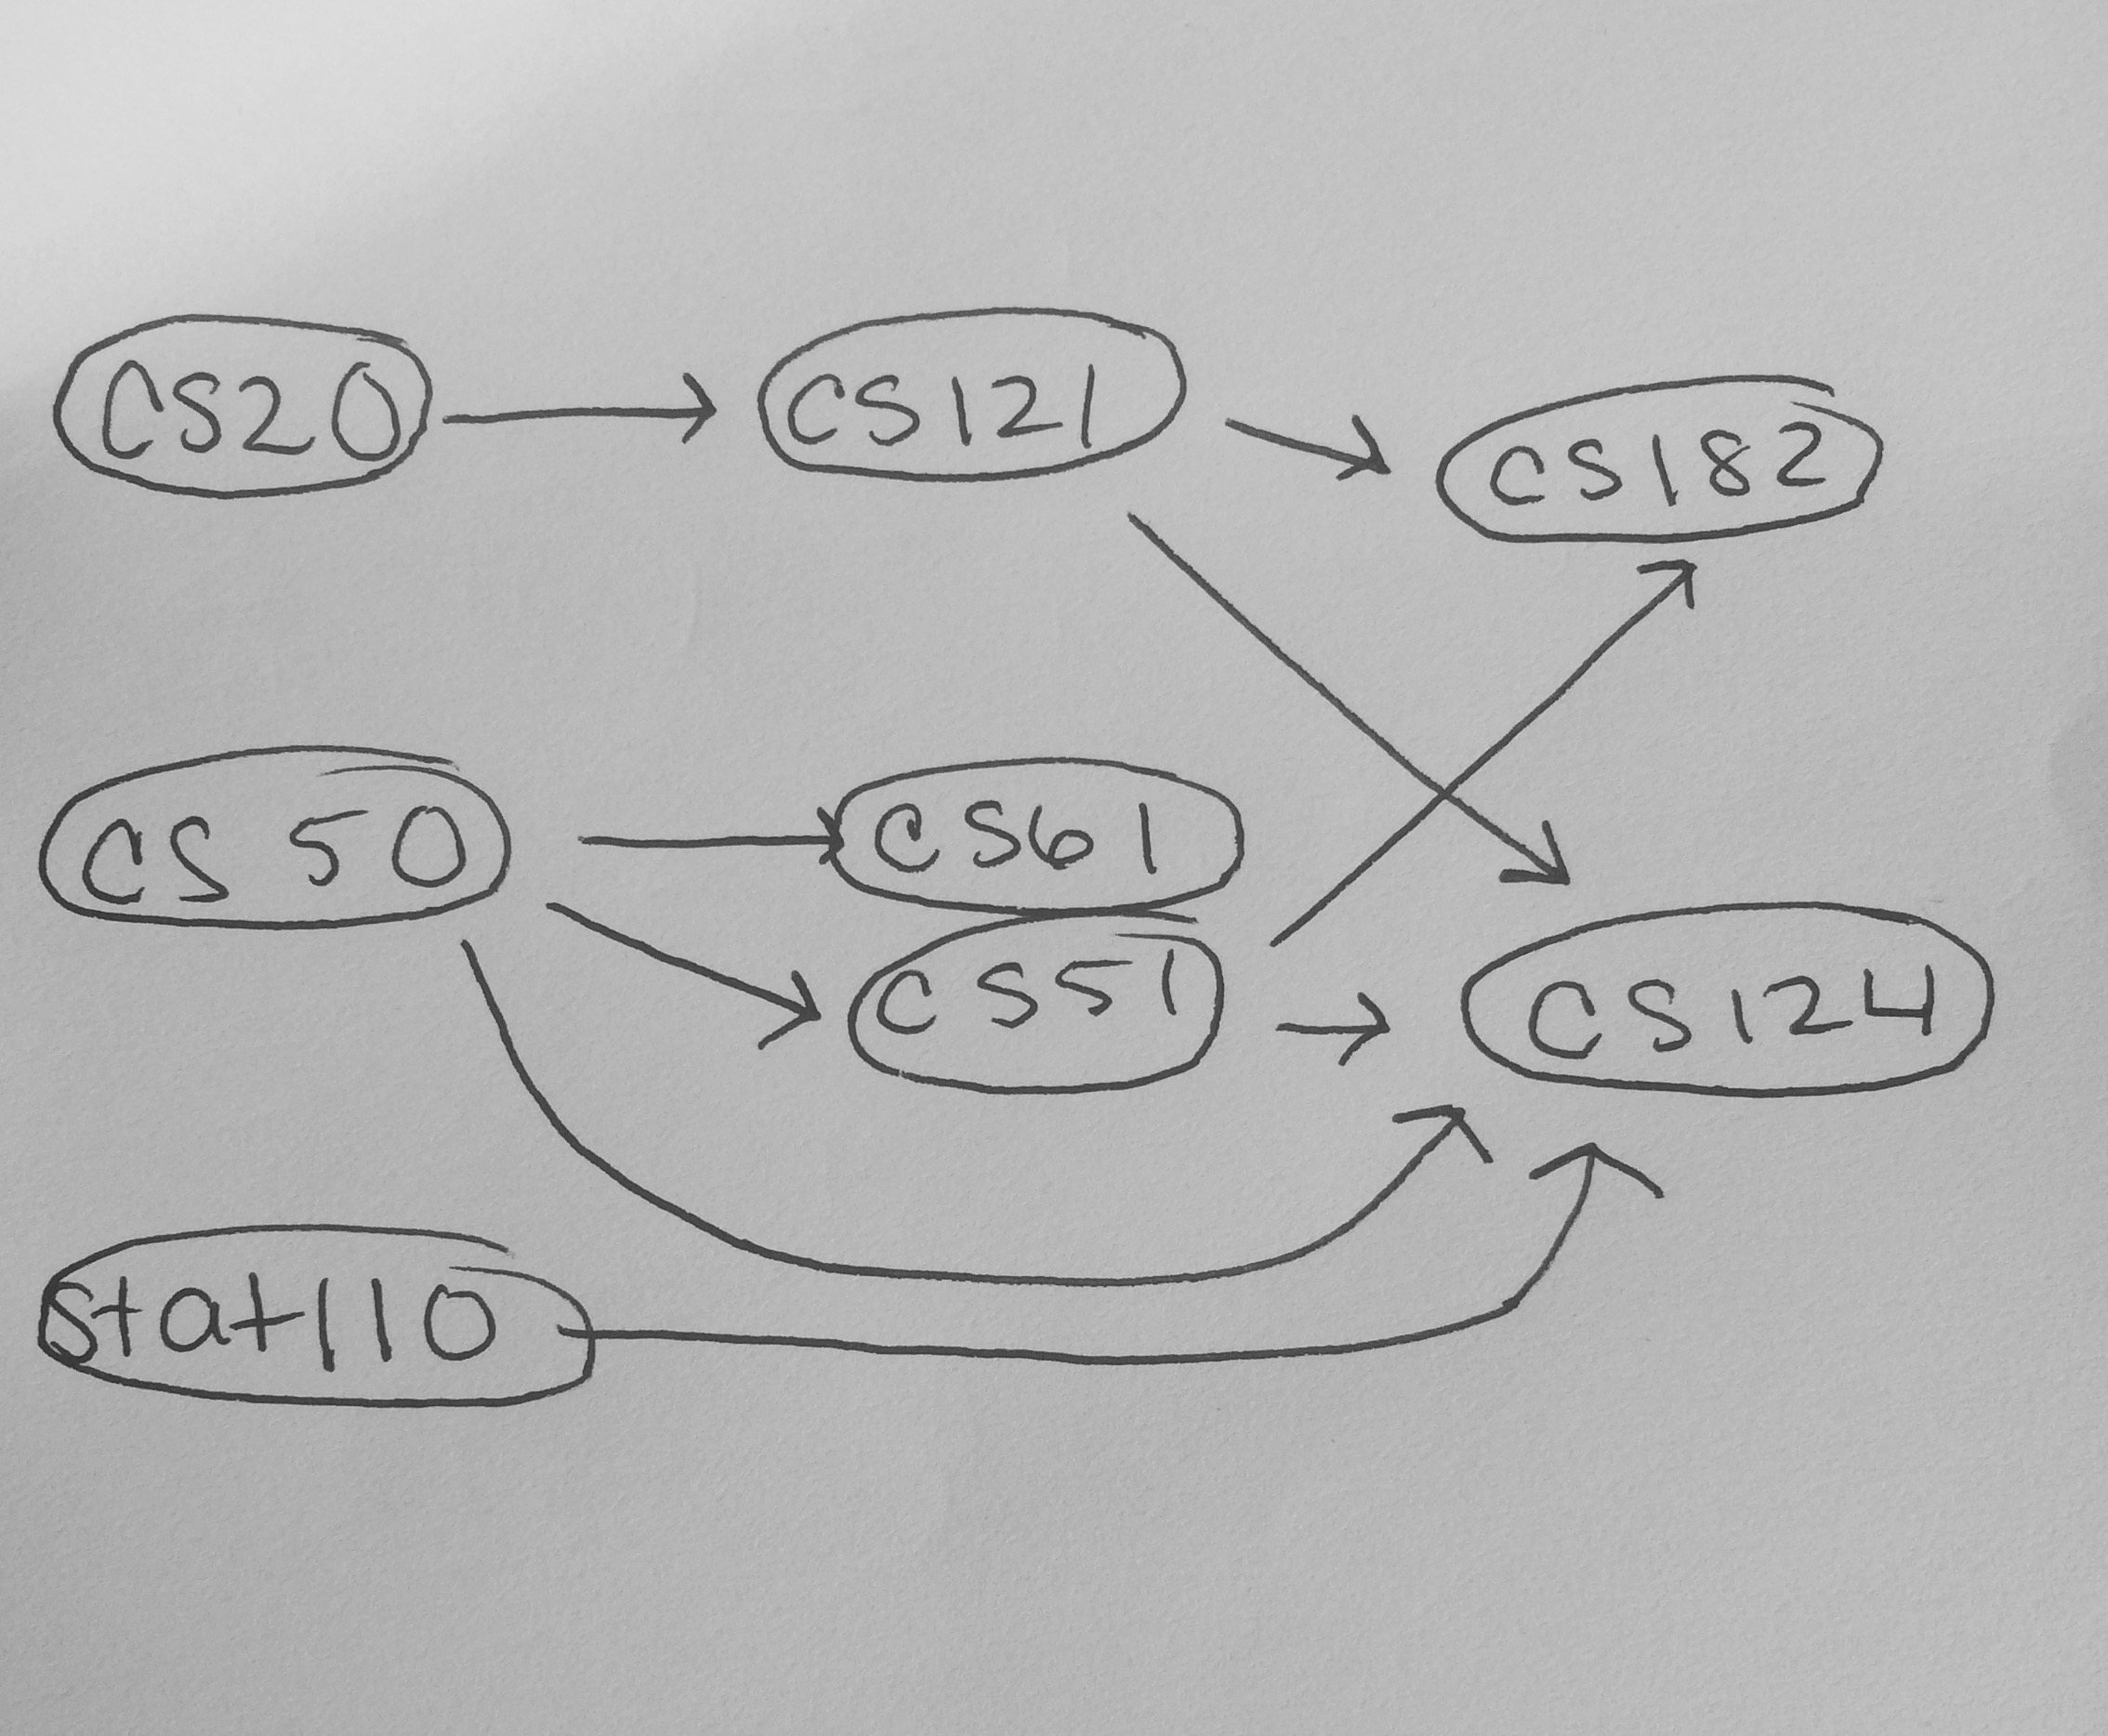
\includegraphics[width=3in]{ClassGraph.jpg}
\subsolution This graph is a DAG. It should not have a cycle because that would make it impossile to successfully construct a schedule; if courses are prerequisites for each other there is no way to start taking courses since there is a barrier to entry for every course. 
\subsolution Three semesters. The first semester we take CS20, CS50, and Stat110. The second semester we take CS121, CS61, and CS51. Third semester we take CS182 and CS124. 


\end{solution}

\problem Prove the triangle inequality, which states that for any $u, x, v \in V$
\[dist(u, v) \le dist(u, x) + dist(x, v)\]
where $dist(u,v)$ is the shortest path between the vertices $u$ and $v$.

\begin{solution}
There are two possible cases: either w is a point on the path from u to v, or it is a point not on the path. If x is on the path, then $dist(u,x) + dist(x,v) = dist(u,v)$, so by definition the inequality holds. If x is not a point on the path from u to v, then we know that $dist(u,v)$ is the shortest path between u and v. Thus, any path that goes through another point must be longer than this path by definition. 
\end{solution}

\problem [BONUS] A topological ordering of a grpah is an ordering of the nodes such that if there is an edge between vertexes a and b in the graph, then a is before b in the topological ordering. Prove that we can provide a topological ordering for any DAG> 

\begin{solution}
Proof by induction. Base case: a single vertex. The topological ordering is just that vertex. Induction: assume we can provide a topological ordering for n vertices. Let us prove this is also the case for $n+1$ vertices. If we insert another vertex into our graph containing n vertexes, let us consider where we will place this new vertex in the topological ordering. If it has only eges coming in, then we can place it at the end of our ordering. If it has only edges going out, we can place it at the beginning. If it has both in and out, we place it in the ordering such that it is after the vertexes that have edges to it and before those it has edges to. Since there is no cycle in the graph, we know we can find such a location without disrupting the topological ordering. 
\end{solution}


\end{document}
